%%%%%%%%%%%%%%%%%%%%%%%%%%%%%%%%%%%%%%%%%%%%%%%%%%%%%%%%%%%%%%%%%%%%%%%%%%%%%%%
% Chapter 3: Procedimiento experimental 
%%%%%%%%%%%%%%%%%%%%%%%%%%%%%%%%%%%%%%%%%%%%%%%%%%%%%%%%%%%%%%%%%%%%%%%%%%%%%%%


%++++++++++++++++++++++++++++++++++++++++++++++++++++++++++++++++++++++++++++++

\section{Procedimiento}
\label{3:sec:1}
El método de la bisección es un proceso iterativo que sigue los siguientes pasos:
\begin{enumerate}
 \item
  Se ''parte'' por la mitad el intervalo [a,b]. Por lo que se cogen los valores de los extremos y se dividen por $2$.
  \begin{center}
   $$ c_1=\frac{a+b}{2} $$
  \end{center}
 \item
  Luego hay que mirar los signos de la función en el punto c y comparar con los signos de la función de los extremos.
   \begin{enumerate}
    \Item
     Si $f(a)*f(c)<0$ se sustituye $c$ por $b$ quedandose $$c_2=\frac{a+c_1}{2}$$
    \Item
     Si $f(b)*f(c)<0$ se sustituye $c$ por $a$ quedandose $$c_2=\frac{c_1+b}{2}$$
   \end{enumerate}
 \item
  Y este proceso se va haciendo hasta que la función en el punto $c_n$ es igual a $0$
 \item
  Hay que tener en cuenta que este método tiene un error y se puede calcular con:
  \begin{center}
   $$ error=\frac{b-a}{2^n} siendo n las veces que se ha partido$$
  \end{center}
\end{enumerate}

%++++++++++++++++++++++++++++++++++++++++++++++++++++++++++++++++++++++++++++++
\section{Programa en Python}
\label{3:sec:2}
Este es el programa hecho en python
\begin{verbatim}
#! encoding: UTF-8
#! /usr/bin/python 

import sin from math

Cero=0.00001

def f(x):
 return sin(x)

def biseccion(a,b,tol):
 c=float((a+b)/2.0)
 while f(c) != Cero) and abs(b-a) > tol:
  if f(a) * f(c) < Cero
   b = c;
  elif f(b) * f(c) < Cero
   a = c;
   c = (a+b)/2.0
  else
   break
 return c

print 'Calcular la raíz de sen de x'
a = float(raw_input('Valor a del intervalo: '))
b = float(raw_input('Valor b del intervalo: '))
t = 0.00000000000001
r = biseccion(a,b,t)
print "El valor de la raíz de seno de x es: %f"%(r)
\end{verbatim}

%------------------------------------------------------------------------------
\begin{figure}[!th]
\begin{center}
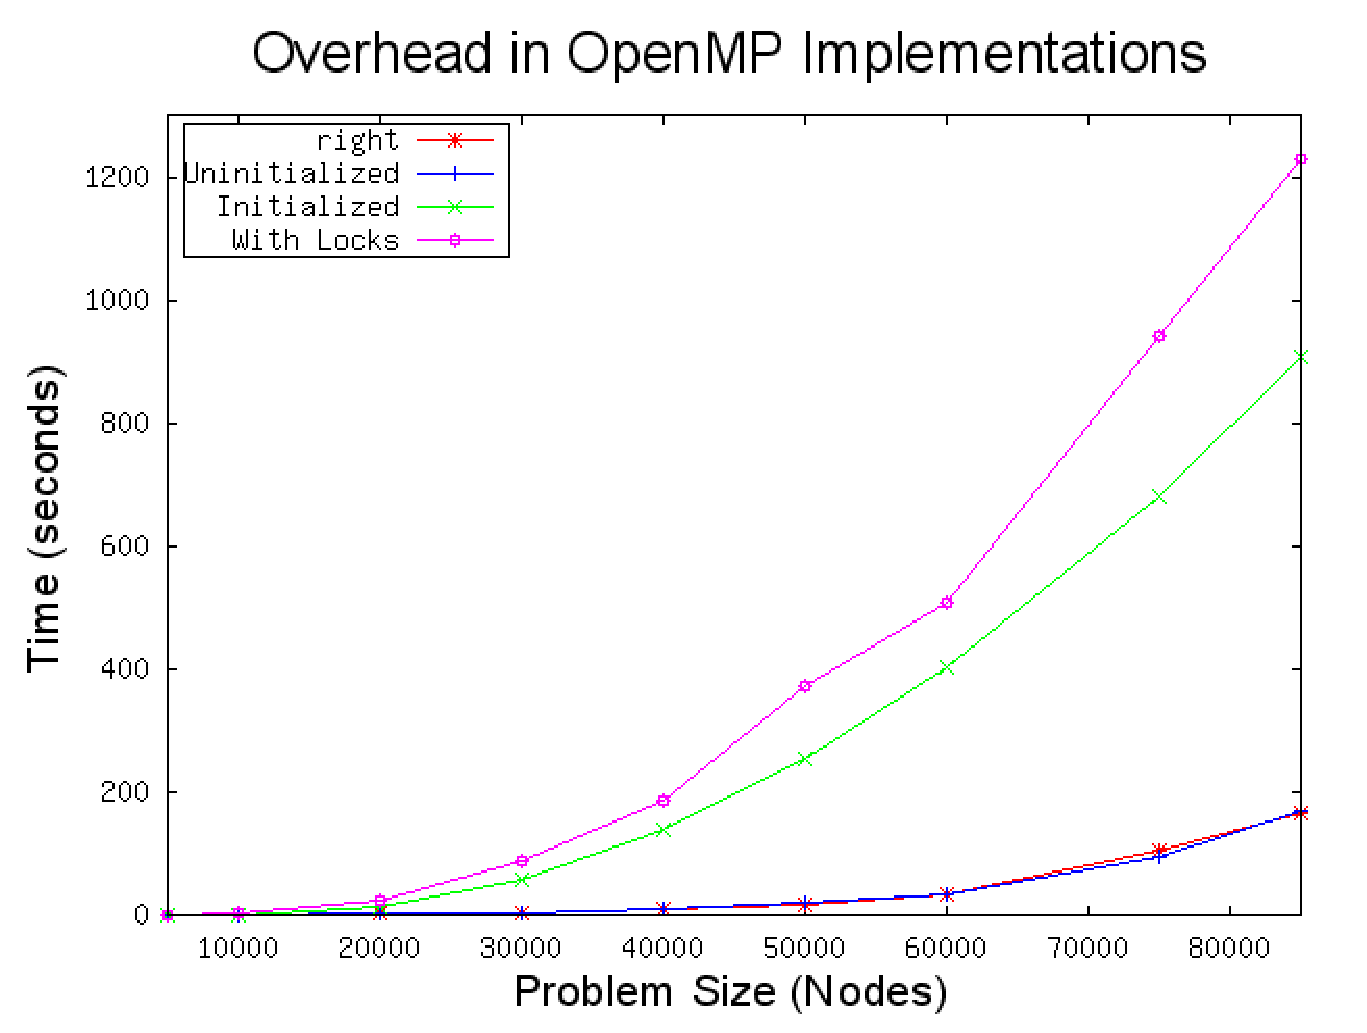
\includegraphics[width=0.75\textwidth]{images/figura1.eps}
\caption{Ejemplo de figura}
\label{fig:1}
\end{center}
\end{figure}
%------------------------------------------------------------------------------


%------------------------------------------------------------------------------
%--------------------------------------------------------------------------
\begin{table}[!ht]
\begin{center}
\begin{tabular}{|c|c|} \hline 
\textbf{Tiempo  } & \textbf{Velocidad} \\ 
\textbf{($\pm$ 0.001 s)} & \textbf{($\pm$ 0.1 m/s)} \\ \hline \hline
1.234 &
67.8
\\
\hline

2.345 &
78.9
\\
\hline

3.456 &
89.1
\\
\hline

4.567 &
91.2
\\
\hline

\end{tabular}
\end{center}
\caption{Resultados experimentales de tiempo (s) y velocidad (m/s)}
\label{tab:1}
\end{table}


%------------------------------------------------------------------------------


